% ===========================================================================
% Figura 1.4: (a) Procedimiento para calcular el retardo de propagación
%             (b) Impacto de la deriva de los relojes
% Basada en la Figura 1.4 del documento base
% ===========================================================================
\documentclass[tikz,border=10pt]{standalone}
\usepackage[utf8]{inputenc}
\usepackage[T1]{fontenc}
\usepackage{lmodern}
\usepackage{amsmath}
\usetikzlibrary{shapes.geometric, arrows.meta, positioning, calc, backgrounds}

\begin{document}
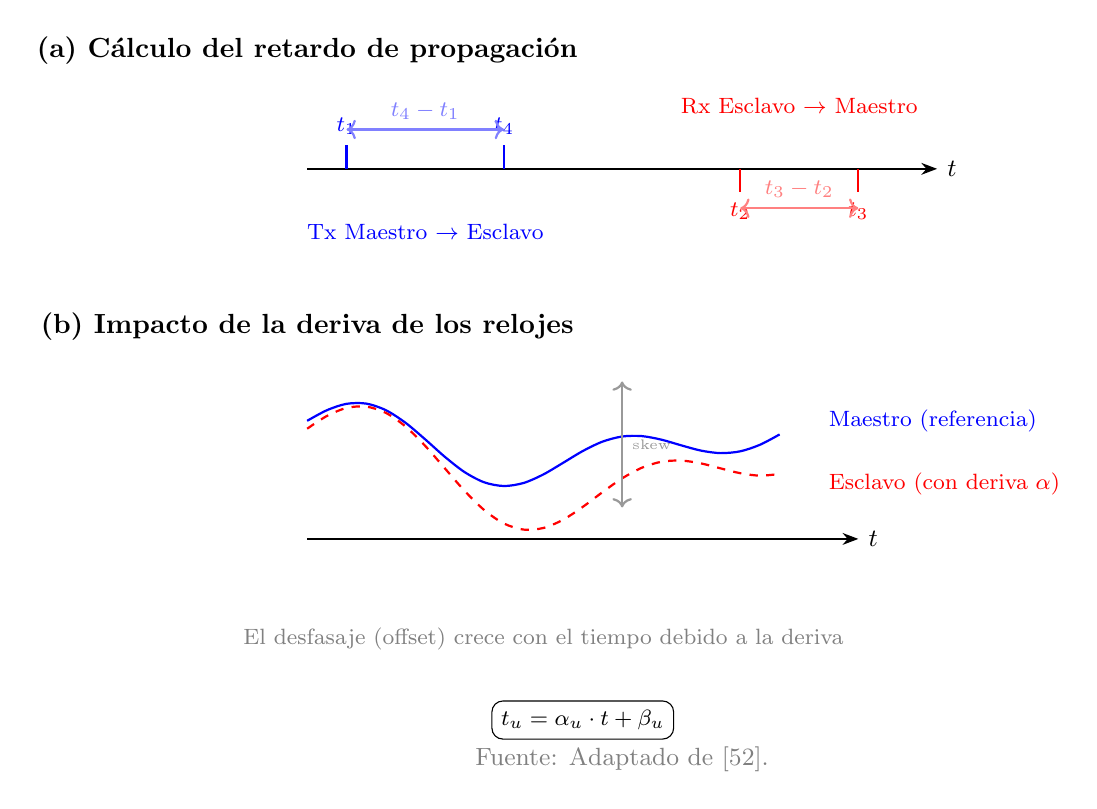
\begin{tikzpicture}[font=\small]

  % ===== (a) CÁLCULO DEL RETARDO =====
  \begin{scope}[local bounding box=a]
    \node[font=\bfseries] at (0,1.5) {(a) C\'alculo del retardo de propagación};

    % Timeline
    \draw[thick, -{Stealth[length=2mm]}] (0,0) -- (8,0) node[right] {$t$};

    % Marcas de tiempo
    \draw[-, thick, blue] (0.5,0) -- (0.5,0.3) node[above, font=\footnotesize] {$t_1$};
    \draw[-, thick, blue] (2.5,0) -- (2.5,0.3) node[above, font=\footnotesize] {$t_4$};
    \draw[-, thick, red] (5.5,0) -- (5.5,-0.3) node[below, font=\footnotesize] {$t_2$};
    \draw[-, thick, red] (7,0) -- (7,-0.3) node[below, font=\footnotesize] {$t_3$};

    % Intervalos
    \draw[<->, thick, blue!50] (0.5,0.5) -- (2.5,0.5) node[midway, above, font=\footnotesize] {$t_4 - t_1$};
    \draw[<->, thick, red!50] (5.5,-0.5) -- (7,-0.5) node[midway, above, font=\footnotesize] {$t_3 - t_2$};

    % Etiquetas de dirección
    \node[font=\footnotesize, blue] at (1.5,-0.8) {Tx Maestro $\rightarrow$ Esclavo};
    \node[font=\footnotesize, red] at (6.25,0.8) {Rx Esclavo $\rightarrow$ Maestro};
  \end{scope}

  % ===== (b) IMPACTO DE LA DERIVA =====
  \begin{scope}[yshift=-3.5cm, local bounding box=b]
    \node[font=\bfseries] at (0,1.5) {(b) Impacto de la deriva de los relojes};

    % Reloj maestro (referencia)
    \draw[thick, blue] plot[domain=0:6, smooth] (\x, {0.3*sin(2*\x r) + 0.3*cos(\x r)});
    \node[blue, right, font=\footnotesize] at (6.5,0.3) {Maestro (referencia)};

    % Reloj esclavo (con deriva)
    \draw[thick, red, dashed] plot[domain=0:6, smooth] (\x, {0.4*sin(1.8*\x r) + 0.5*cos(0.9*\x r) - 0.3});
    \node[red, right, font=\footnotesize] at (6.5,-0.5) {Esclavo (con deriva $\alpha$)};

    % Eje temporal
    \draw[thick, -{Stealth[length=2mm]}] (0,-1.2) -- (7,-1.2) node[right] {$t$};

    % Flecha skew
    \draw[<->, thick, black!40] (4,0.8) -- (4,-0.8) node[midway, right, font=\tiny] {skew};

    \node[font=\footnotesize, text=gray, below] at (3,-2.2) {El desfasaje (offset) crece con el tiempo debido a la deriva};

    % Ecuación
    \node[draw, fill=white, rounded corners, font=\footnotesize] at (3.5,-3.5) {$t_u = \alpha_u \cdot t + \beta_u$};
  \end{scope}

  \node[font=\small, text=gray] at (4,-7.5) {Fuente: Adaptado de [52].};
\end{tikzpicture}
\end{document}
